\documentclass[aspectratio=169]{beamer}
\usepackage{tabularx}
\usepackage{graphicx}
\usepackage{eso-pic}

\usepackage{minted}
\usepackage{hyperref}
\usepackage{animate}

\usepackage{tcolorbox}

\makeatletter
\newenvironment{myitemize}{%
   \setlength{\topsep}{0pt}
   \setlength{\partopsep}{0pt}
   \renewcommand*{\@listi}{\leftmargin\leftmargini \parsep\z@ \topsep\z@ \itemsep\z@}
   \let\@listI\@listi
   \itemize
}{\enditemize}
\makeatother

\graphicspath{{img/}}

\usetheme{Warsaw}
\usemintedstyle{monokai}

\setbeamercolor{normal text}{fg=white,bg=black!90}
\setbeamercolor{structure}{fg=white}
\setbeamercolor{alerted text}{fg=red!85!black}
\setbeamercolor{item projected}{use=item,fg=black,bg=item.fg!35}
\setbeamercolor*{palette primary}{use=structure,fg=structure.fg}
\setbeamercolor*{palette secondary}{use=structure,fg=structure.fg!95!black}
\setbeamercolor*{palette tertiary}{use=structure,fg=structure.fg!90!black}
\setbeamercolor*{palette quaternary}{use=structure,fg=structure.fg!95!black,bg=black!80}
\setbeamercolor*{framesubtitle}{fg=white}
\setbeamercolor*{block title}{parent=structure,bg=black!60}
\setbeamercolor*{block body}{fg=black,bg=black!10}
\setbeamercolor*{block title alerted}{parent=alerted text,bg=black!15}
\setbeamercolor*{block title example}{parent=example text,bg=black!15}
\setbeamertemplate{navigation symbols}{}
\setbeamercolor{footercolor}{fg=white,bg=black}

\makeatletter
\defbeamertemplate*{footline}{myfootline}
{
  \leavevmode%
  \hbox{%
  \begin{beamercolorbox}[wd=.333333\paperwidth,ht=2.25ex,dp=1ex,center]{footercolor}%
    \insertshorttitle
  \end{beamercolorbox}%
  \begin{beamercolorbox}[wd=.333333\paperwidth,ht=2.25ex,dp=1ex,center]{footercolor}%
    \insertshortauthor\expandafter\beamer@ifempty\expandafter{\beamer@shortinstitute}{}{~~(\insertshortinstitute)}
  \end{beamercolorbox}%
  \begin{beamercolorbox}[wd=.333333\paperwidth,ht=2.25ex,dp=1ex,right]{footercolor}%
    \insertshortdate{}\hspace*{2em}
    \insertframenumber{} / \inserttotalframenumber\hspace*{2ex} 
  \end{beamercolorbox}}%
  \vskip0pt%
}
\makeatother

\title{Girls PowerTech - Google Chrome Malware}

\institute{GoSecure}
\author{Lilly Chalupowski and Xandria Richman}
\date{May 3, 2018}

\begin{document}

\setbeamertemplate{footline}{}
\begin{frame}[t]
  \begin{center}
    \begingroup
    \fontsize{20pt}{20pt}\selectfont
    \inserttitle \\
    \endgroup
    \bigskip
      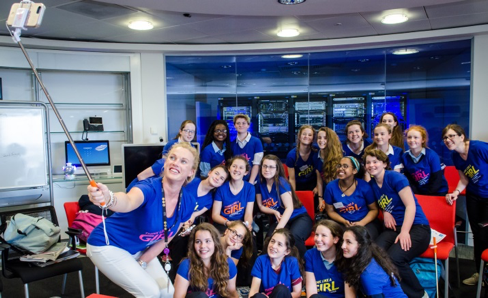
\includegraphics[scale=1]{title} \\
    \bigskip
    \insertauthor \\
    \insertdate
  \end{center}
\end{frame}

\newcommand\AtPagemyUpperLeft[1]{\AtPageLowerLeft{%
\put(\LenToUnit{0.94\paperwidth},\LenToUnit{0.93\paperheight}){#1}}}
\AddToShipoutPictureFG{
  \AtPagemyUpperLeft{{
\includegraphics[width=1cm,keepaspectratio]{gosecure}}}
}%

\setbeamertemplate{footline}[myfootline]

\begin{frame}
  \frametitle{Introduction}
  \begin{center}
    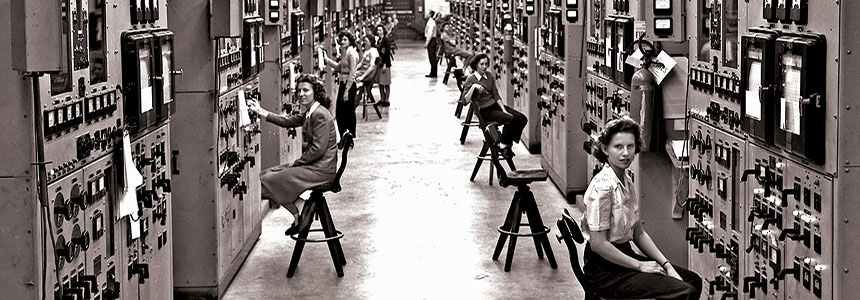
\includegraphics[scale=0.4]{women_in_tech}
  \end{center}
\end{frame}

\begin{frame}
  \frametitle{Xandria Richman}
  \begin{columns}
    \begin{column}{0.5\textwidth}
      
\includegraphics[scale=0.33]{xandria_richman}
    \end{column}
    \begin{column}{0.5\textwidth}
      \begin{center}
        \begin{tcolorbox}[title=Biography,colback=gray]
          \begin{itemize}
            {\color{black} \tiny
            \item Bachelor of Computer Science from UNB
            \item Volunteered for UNB to help introduce girls to technology
            \item Joined GoSecure in 2016 and has obtained a leadership position
            \item Found Flaws in Canada-wide loyalty card program
            \item Previously worked at Siemens Canada and IBM
            }
          \end{itemize}
        \end{tcolorbox}
      \end{center}
    \end{column}
  \end{columns}
\end{frame}

\begin{frame}
  \frametitle{Lilly Chalupowski}
  \begin{columns}
    \begin{column}{0.5\textwidth}
      
\includegraphics[scale=0.5]{lilly_chalupowski}
    \end{column}
    \begin{column}{0.5\textwidth}
      \begin{center}
        \begin{tcolorbox}[title=Biography,colback=gray]
          \begin{itemize}
            {\color{black} \tiny
            \item Studied Computer Science and Audio Engineering at Acadia University
            \item Almost 100\% self taught on programming and hacking
            \item Presented at AtlSecCon on ROP Chain Exploitation
            \item Presented at AtlSecCon on Google Chrome Malware
            \item Taught SQL Injection and Phishing Awareness to Digital Nova Scotia Discovery Camp Kids
            \item Volunteers for Techsploration and mentoring girls looking to enter the tech industry
            \item Badger - ASLR Entropy and PE File Security Enumerator
            \item Chameleon - Custom Base64 Encoder
            \item Chrome Crusader - Google Chrome Malware and Botnet
            }
          \end{itemize}
        \end{tcolorbox}
      \end{center}
    \end{column}
  \end{columns}
\end{frame}

\begin{frame}
  \frametitle{Disclaimer}
  \framesubtitle{Stay Alert Stay Safe}
  \begin{tcolorbox}[title=disclaimer.log,colback=gray]
    The tools and techniques covered in this presentation can be dangerous and are\\
    being shown for educational purposes.\\
    \newline
    It is a violation of Federal laws to attempt gaining unauthorized access to information, assets or systems belonging to others, or to exceed authorization on systems for which you have not been granted.\\
    \newline
    Only use these tools with/on systems you own or have written permission from the owner. We (the speakers) do not assume any responsibility and shall not be held liable for any illegal use of these tools.\\
  \end{tcolorbox}
\end{frame}

\begin{frame}
  \frametitle{What is Malware}
  \begin{center}
    \animategraphics[loop,controls,scale=0.4]{10}{img/malware/malware-}{0}{15}
    \begin{tcolorbox}[title=\href{https://en.wikipedia.org/wiki/Malware}{Definition of Malware},colback=gray]
      Software that is intended to damage or disable computers and computer systems.
    \end{tcolorbox}
  \end{center}
\end{frame}

\begin{frame}
  \frametitle{Google Chrome}
  \begin{columns}
    \begin{column}{0.5\textwidth}
      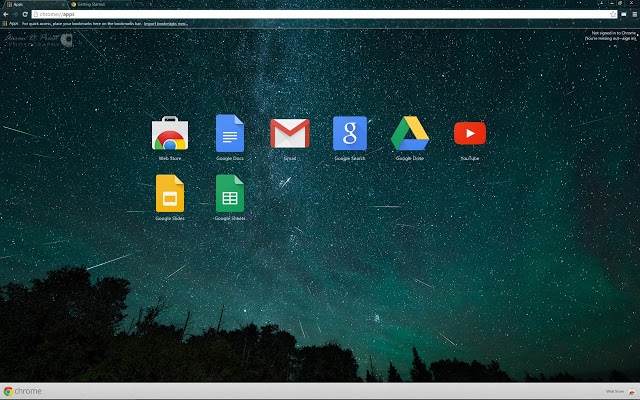
\includegraphics[scale=0.32]{google_chrome}
    \end{column}
    \begin{column}{0.5\textwidth}
      \begin{center}
        \begin{tcolorbox}[title=\href{https://en.wikipedia.org/wiki/Google_Chrome}{Google Chrome},colback=gray]
          {\small A freeware web browser developed by Google.}
        \end{tcolorbox}
      \end{center}
    \end{column}
  \end{columns}
\end{frame}

\begin{frame}
  \frametitle{Malware Inside Google Chrome}
  \framesubtitle{How is it possible?}
  \begin{center}
    
\includegraphics[scale=0.2]{how}
  \end{center}
\end{frame}

\begin{frame}
  \frametitle{Google Chrome Extensions}
  \framesubtitle{Which one is Malware?}
  \begin{center}
    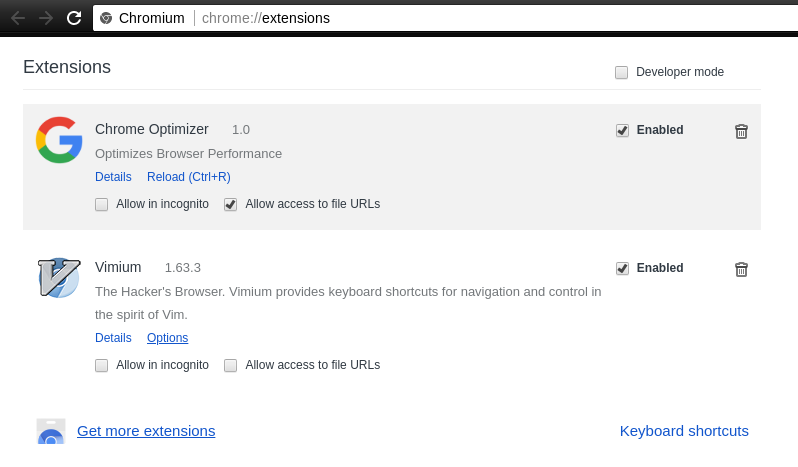
\includegraphics[scale=0.3]{extensions}
  \end{center}
\end{frame}

\begin{frame}
  \frametitle{How does it Work?}
  \begin{center}
    \begin{itemize}
    \item Access All Page Data
    \item Bypass Security Headers
    \item AJAX Requests
    \end{itemize}
  \end{center}
\end{frame}

\begin{frame}
  \frametitle{Accessing All Page Data}
  \begin{center}
    \begin{itemize}
    \item Extensions live inside the browser
    \item Able to access the DOM (rendered page data)
    \item Works on HTTP as well as HTTPS websites (includes banking websites)
    \item Steals information
      \begin{itemize}
      \item Usernames
      \item Passwords
      \item Cookies
      \item IP Address
      \item Conversations
      \end{itemize}
    \end{itemize}
  \end{center}
\end{frame}

\begin{frame}
  \frametitle{Bypass Security Headers}
  \begin{center}
      \begin{tcolorbox}[title=Security Header Definition,colback=gray]
        Data that exists within the HTTP protocol as headers that is sent by a server to a browser to invoke security policies.
      \end{tcolorbox}
      \begin{itemize}
      \item Feature is built in
      \item Allows modification of security headers
      \item Part of Google's Custom JavaScript Extension API
      \end{itemize}
  \end{center}
\end{frame}

\begin{frame}
  \frametitle{AJAX Requests}
  \begin{center}
    \begin{tcolorbox}[title=\href{https://en.wikipedia.org/wiki/Ajax_(programming)}{AJAX Definition},colback=gray]
      With Ajax, Web applications can send and retrieve data from a server asynchronously (in the background) without interfering with the display and behavior of the existing page.
    \end{tcolorbox}
    \begin{itemize}
    \item Send data back and forth in the background
    \item Execute commands based on the data you receive
    \end{itemize}
  \end{center}
\end{frame}

\end{document}